%ws6.tex
%notes for the course Mathematics for Computer Science A COMS10014
%taught at the University of Bristol
%2020_21 Conor Houghton conor.houghton@bristol.ac.uk

%To the extent possible under law, the author has dedicated all copyright 
%and related and neighboring rights to these notes to the public domain 
%worldwide. These notes are distributed without any warranty. 


\documentclass[11pt,a4paper]{scrartcl}
\typearea{12}
\usepackage{graphicx}
%\usepackage{pstricks}
\usepackage{listings}
\usepackage{color}
\usepackage{tikz}
\usetikzlibrary{decorations.markings}
\lstset{language=C}
\usepackage{fancyhdr}
\pagestyle{fancy}
\lhead{\texttt{cs-uob.github.io/COMS10014/ and github.com/coms10011/2021\_22}}
\lfoot{COMS10014 - P\&C ws8 - Conor}
\begin{document}

\section*{Probability and Combinatorics Worksheet 8 - solutions}


\subsection*{Questions}

These are the questions you should make sure you work on in the workshop.

\begin{enumerate}


\item The length of human pregnancies from conception to birth
  approximates a normal distribution with a mean of 266 days and a
  standard deviation of 16 days.  What proportion of all pregnancies
  will last between 240 and 270 days (roughly between 8 and 9 months)?
\\ \\ \\
\textbf{Solution}:
So
\begin{equation}
  z_1=\frac{240-266}{16}=-1.625/\sqrt{2}\approx-1.15
\end{equation}
and
\begin{equation}
  z_2=\frac{270-266}{16}=0.25/\sqrt{2}=\approx 0.18
\end{equation}
giving
\begin{equation}
  p(\mbox{between 250 and 270})=\frac{1}{2}[\mbox{erf}\,(0.18)-\mbox{erf}\,(-1.15)]\approx 0.55
\end{equation}


\item Starting from the expression for the mean
  \begin{equation}
    \mu=\frac{1}{\sqrt{2\pi\sigma^2}}\int_{-\infty}^\infty xe^{-\frac{(x-\mu)^2}{2\sigma^2}}dx
  \end{equation}
  show the Gau\ss{}ian distribution has variance $\sigma^2$.
\\ \\ \\
\textbf{Solution}: Differenciate with respect to $\mu$ to get
\begin{equation}
  1=\frac{1}{\sqrt{2\pi\sigma^2}}\int_{-\infty}^\infty x\frac{x-\mu}{\sigma^2}e^{-\frac{(x-\mu)^2}{2\sigma^2}}dx
\end{equation}
and multiply across by the $\sigma^2$ to get
\begin{equation}
  \sigma^2=\frac{1}{\sqrt{2\pi\sigma^2}}\int_{-\infty}^\infty x(x-\mu)e^{-\frac{(x-\mu)^2}{2\sigma^2}}dx
\end{equation}
and then a bit of algebra gives
\begin{equation}
  \sigma^2=\frac{1}{\sqrt{2\pi\sigma^2}}\int_{-\infty}^\infty x^2e^{-\frac{(x-\mu)^2}{2\sigma^2}}dx-\mu\frac{1}{\sqrt{2\pi\sigma^2}}\int_{-\infty}^\infty xe^{-\frac{(x-\mu)^2}{2\sigma^2}}dx
\end{equation}

\item The size of a standard croquet ball is 3 5/8
  inches\footnote{Everything in croquet is measured in old timey
    units}. The height of a croquet hoop is 3 3/4 inches. If a not
  very good croquet-ball making machine makes croquet balls whose mean
  matches the standard and with standard deviation 1/8 inch, what is
  the chance it will make a ball too large to fit through the hoop?
  You can write the solution in terms of the error function.
  \\ \\ \\ \textbf{Solution}: So
\begin{equation}
z=\frac{x-\mu}{\sqrt{2}\sigma}
\end{equation}
so for $x_1=3.75$ in, we have
\begin{equation}
z_1=\frac{1/8}{\sqrt{2}/8}=\frac{1}{\sqrt{2}}
\end{equation}
Any height bigger than this will not fit, so $z_2=\infty$ and $\mbox{erf}{\infty}=1$ so
\begin{equation}
\mbox{Prob}(x>3.75)=\frac{1}{2}[1-\mbox{erf}(1/\sqrt{2})]\approx 0.16
\end{equation}
where the 0.16 is given for interest, it wasn't expected as part of the answer.

  

\item If $X$ and $Y$ are two independent random variables what is var$(X+Y)$?
 \\ \\ \\
\textbf{Solution}: So, using the obvious notation 
\begin{equation}
  \mbox{var}(X+Y)=\langle (X+Y)^2\rangle -(\mu_X+\mu_Y)^2
\end{equation}
or
\begin{equation}
  \mbox{var}(X+Y)=\langle X^2\rangle +2\langle XY\rangle +\langle Y^2\rangle -\mu_X^2-2\mu_x\mu_Y+\mu_Y^2
\end{equation}
and by independence $\langle XY\rangle=\langle X\rangle\langle Y\rangle=\mu_X\mu_Y$ giving
\begin{equation}
  \mbox{var}(X+Y)=\mbox{var}(X)+\mbox{var}(Y)
\end{equation}



\end{enumerate}

\subsection*{Extra questions}

\begin{enumerate}

  
\item This will look like a long question but it is almost all
  background and the question is not too bad when you actually read
  through it. In particle physics when a collider is being used to
  find a new particle like the Higgs boson or the top squark
  scientists don't detect the sought after particle directly since it
  usually decays almost straight away, instead they detect the more
  common particles that particle will decay into, for example, a Higgs
  boson can decay in to two photons and these can be detected. Roughly
  speaking scientists count these events. However, the whole situation
  is very messy and there will always be some events even if the
  particle doesn't exist at the energy being examined. The amount of
  these background events will fluctuate from experiment to
  experiment, typically like a Gau\ss{}ian. The scientific team is
  allowed to claim they have discovered the particle if the number of
  events they measure is more than five standard deviations above
  what would be expected if the particle didn't exist. What is the
  probability of this \lq{}discovery\rq{} happening by chance?
  \\ \\ \\ \textbf{Solution}: So we are interested in the probability of a results bigger than $\mu+5\sigma$. Now
\begin{equation}
z_1=\frac{\mu+5\sigma-\mu}{\sqrt{2}\sigma}=\frac{5}{\sqrt{2}}
\end{equation}
and
\begin{equation}
\mbox{Prob}(x>\mu+5\sigma)=\frac{1}{2}[1-\mbox{erf}(5/\sqrt(2))]
\end{equation}
which is about one chance in 3.5 million.
    
\item Australorp hens weigh on average 4kg with a standard deviation
  0.25kg; in one farm australorps who weigh less than 3.5kg are fed
  \textsl{patent chicken spicer}, a mixture of chalk, corn and
  pepper. What fraction of these hens are fed patent chicken spicer?
  \\ \\ \\ \textbf{Solution}: Here is a picture of one of my hens, an Australorp, sitting on the kitchen window ledge.
  \begin{center}
    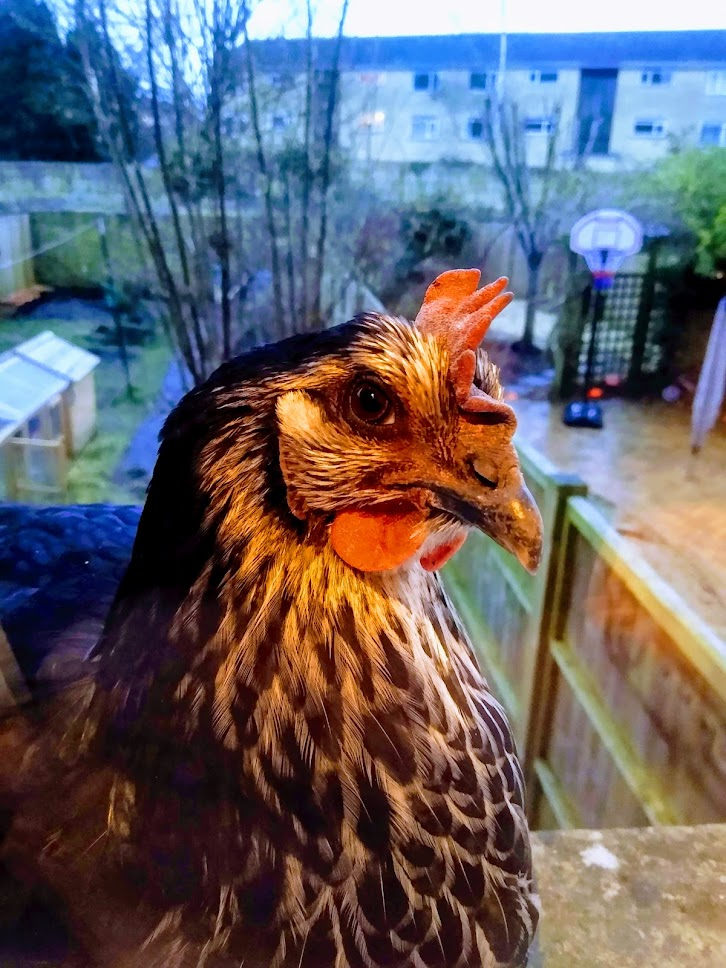
\includegraphics[width=8cm]{hen.jpg}
  \end{center}
  So we are asking for $P(x<3.5)$ and since
  $$z=\frac{3.5-4}{0.25\sqrt{2}}=\sqrt{2}$$
    the probability, and hence the proportion, is
    $$P(x<3.5)=\frac{1}{2}[1-\mbox{erf}\,(\sqrt{2})]\approx 0.02275$$

    
\item The Beta distribution for a random variable $X$ has non-zero probability for $x\in(0,1)$ and probability mass function
  \begin{equation}
    p(x)=\frac{1}{B(\alpha,\beta)}x^{\alpha-1}(1-x)^{\beta-1}
  \end{equation}
  where $\alpha$ and $\beta$ are shape parameters and $B(\alpha,\beta)$ is the Beta function, a special function\footnote{Roughly speaking, in mathematics a special function is an integral or solution to a differential equation that could not, in the nineteenth century, be related to a function that had already been names, so instead it is given a name of its own} be defined as
  \begin{equation}
    B(\alpha,\beta)=\int_0^1 x^{\alpha-1}(1-x)^{\beta-1}
  \end{equation}
  and serves to normalize the distribution so $\int_0^1{p(x)dx} =1$. With some fiddling with the integrals and some integrating by parts you can show
  \begin{equation}
    B(\alpha,\beta)=B(\alpha+1,\beta)+B(\alpha,\beta+1)
  \end{equation}
  and from this it follows, again you don't need to show this, that
  \begin{equation}
    B(\alpha+1,\beta)=\frac{\alpha}{\alpha+\beta}B(\alpha,\beta)
  \end{equation}
  Find the mean of the Beta distribution.
  \\ \\ \\ \textbf{Solution}:
  So
  \begin{equation}
    \mu=\frac{1}{B(\alpha,\beta)}\int_0^1 x x^{\alpha-1}(1-x)^{\beta-1}dx=\frac{1}{B(\alpha,\beta)}\int_0^1 x^{(\alpha+1)-1}(1-x)^{\beta-1}dx=\frac{B(\alpha+1,\beta)}{B(\alpha,\beta)}
  \end{equation}
  so
  \begin{equation}
    \mu=\frac{\alpha}{\alpha+\beta}
  \end{equation}

 
\item This is going to be complicated but it introduces the concept of
  a conjugate prior, so bear with me! You go to a casino, the
  Baysiana, and the slot machines have a probability $x$ of paying
  out. You don't know this probability because it varies from casino
  to casino, in fact as an international gambler you have been to many
  casinos and you know that the distribution of $x$ for casinos
  satisfies a Beta distribution with some $\alpha$ and $\beta$ you
  have calculated from your many casino visits. In other words your
  prior for the slot machines at the Baysiana, before you play one, is
  \begin{equation}
    p(x)\sim \mbox{Beta}(\alpha,\beta)
  \end{equation}
  or
  \begin{equation}
    p(x)=\frac{1}{B(\alpha,\beta)}x^{\alpha-1}(1-x)^{\beta-1}
  \end{equation}
  and $\alpha$ and $\beta$ describe your understanding of what $p$ is
  for the Baysiana. Now you put a coin in and pull the lever, you win!
  What is your posterior distribution for $x$?
  \\ \\ \\ \textbf{Solution}:
  So we want $p(x|w)$ where $w$ is a win and hence, by definition $p(w|x)=x$. We use the usual rule
  \begin{equation}
    p(x|w)=\frac{p(w|x)p(x)}{p(w)}
  \end{equation}
  where $p(x)$ is the original prior so
  \begin{equation}
    p(x|w)=\frac{x x^{\alpha-1}(1-x)^{\beta-1}}{B(\alpha,\beta)p(w)}
  \end{equation}
  now
  \begin{equation}
    p(w) = \int_0^1 p(w|x)p(x)dx
  \end{equation}
  or
  \begin{equation}
    p(w)=\frac{1}{B(\alpha,\beta)}\int_0^1 x^{\alpha}(1-x)^{\beta-1}dx=\frac{B(\alpha+1,\beta)}{B(\alpha,\beta)}
  \end{equation}
  Hence
  \begin{equation}
    p(x|w)=\frac{x^{(\alpha+1)-1}(1-x)^{\beta-1}}{B(\alpha+1,\beta)}
  \end{equation}
  or
  \begin{equation}
    p(x|w)\sim \mbox{Beta}(\alpha+1,\beta)
  \end{equation}
This means the consequence of winning is to change your prior by adding one to $\alpha$! 

  
  

  
\end{enumerate}

\end{document}

